\documentclass[10pt,twocolumn,letterpaper]{article}

\usepackage{cvpr}
\usepackage{times}
\usepackage{cite}
\usepackage{epsfig}
\usepackage{graphicx}
\usepackage{amsmath}
\usepackage{amssymb}

\usepackage[pagebackref=true,breaklinks=true,letterpaper=true,colorlinks,bookmarks=false]{hyperref}

\cvprfinalcopy % *** Uncomment this line for the final submission

\def\cvprPaperID{****} % *** Enter the CVPR Paper ID here
\def\httilde{\mbox{\tt\raisebox{-.5ex}{\symbol{126}}}}

\ifcvprfinal\pagestyle{empty}\fi
\setcounter{page}{1}

\begin{document}

\author{Qingyun Li\\\\
August 10, 2018}        
\title{Underwater Image Restoration}

\maketitle

\section{Introduction}
\par Restoring underwater image is similar to restoring haze image, they are known to be ill-posed. Images captured underwater are usually degraded due to the effects of absorption and scattering. Degraded underwater images show some limitations when they are uesd for display and analysis. Because underwater images with low contrast and color cast decrease the accuracy rate of underwater object detection and marine biology recognition. To overcome those limitations, the authors proposed a systematic underwater image enhancement methods which includes an underwater image dehazing algorithm and a contrast enahncement algorithm~\cite{Li2016Underwater}. Built on a minimum information loss principle, an effective underwater image dehazing algorithm is proposed to restore the visibility, color and natural appearance of underwater images. 
\section{Ralated work}
\par Numerous underwater image enhancement and restoration methods have emerged in the last few years. Traditional image enhancement methods, like histogram equalization, CLAHE, generalized unsharp masking are effective for common images. However, traditional image enhancement methods can not adaptively compensate the contrast degradation of underwater images. We found that direct applying traditional image enhancement methods to degraded underwater images ignores the fact that contrast degradation of underwater images is proportional to the ditance of object-camera. And the propagation of light in the water is shown at the Figure.~\ref{pro}.
\begin{figure}[htbp]
	\begin{center}
		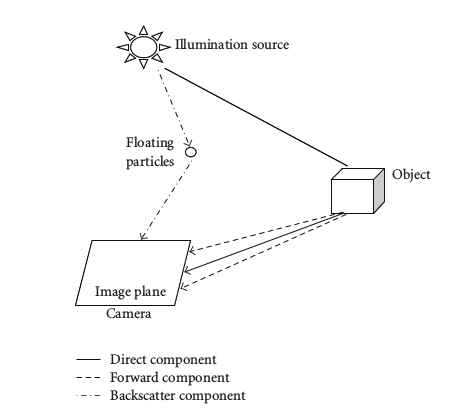
\includegraphics[scale=0.2]{propagation.png}
	\end{center}
	\caption{Propagation of Light in the Water}
	\label{pro}
\end{figure}
\par  We all know the dark channel prior proposed by Kaimming He, it is used to single haze removal. And several methods are based on the extension and modification of He's method which could used to underwater image restoration. But because the wavelength of red light is long, so the red light is disappeared when the depth of water is more than five meters, as is shown at Figure.~\ref{light}. So when we use the dark channel prior to do the underwater image restoration, we acquire the dark channel just from the green and blue channel. 
\begin{figure}[htbp]
	\begin{center}
		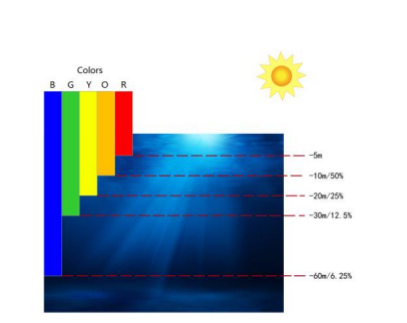
\includegraphics[scale=0.2]{light.png}
	\end{center}
	\caption{Schematic of Light Absorption.}
	\label{light}
\end{figure}

\section{DCP}
\par Recently, I read a paper which apply the dark channel prior to underwater image restoration, and in order to solve the problem which proposed at the last segment, the authors proposed a method corrected the red channel which can be interpreted as a variant of the dark channel method used for images degraded by the atmosphere when exposed to haze.
\par The main model is the transmission estimate from Red Channel, and in this paper, t(x) is estimated as:
\begin{equation}
\begin{aligned}
\tilde{t}(x) = 1-min(\frac{min\limit_{y\in\Omega(x)}(1-I^{R}(y))}{1-A^{R}}, \frac{min\limit_{y\in\Omega(x)}I^{G}(y)}{A^{G}},\\ \frac{min\limit_{y\in\Omega(x)}I^{B}(y)}{A^{B}}) 
\end{aligned}
\end{equation}
\par In fact, there is another method which is estimate the transmission from the green and the blue channel, and in order to compare the red-channel correction and this method, I reappeared the code and acquire the outcome, we can see it at the Figure.~\ref{rc} and \ref{dcp}:
\begin{figure}[htbp]
		\centering{}
		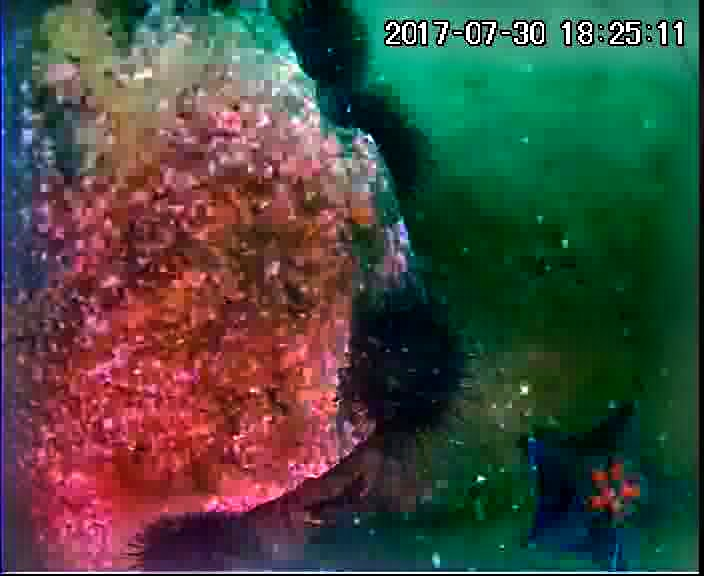
\includegraphics[width=0.9\linewidth]{dcp.jpg}\\
		\caption{DCP outcome}
		\label{dcp}
\end{figure}
\begin{figure}
		\centering{}
		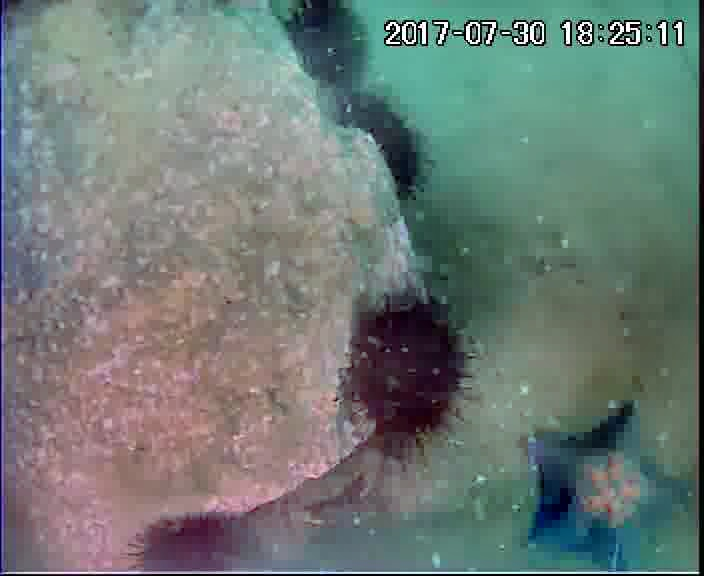
\includegraphics[width=0.9\linewidth]{dcp(rc).jpg}\\
		\caption{Red-Channel correction outcome}
		\label{rc} 	
\end{figure}
\par We can see that after the red-channel corection, the red rock phenomenon has disappeared, and the holistic color is less green, the edge is more clearly. So I think this method may be more useful than dcp when we do the object detection.
  \bibliographystyle{ieee}
  \bibliography{single}
\end{document}